\chapter{Grundlagen}\label{ch:Grundlagen}

In diesem Kapitel werden einige grundlegende Begriffe erklärt und voneinander abgegrenzt, welche für das Verständnis dieser Thesis wichtig sind und sonst für Verwirrung sorgen könnten.

\section{Begrifflichkeiten und Definitionen}\label{Definitionen}

Im Verlauf der Thesis werden einige Begriffe immer wieder verwendet werden die eine feste Definition innerhalb dieser Thesis haben und nicht verwechselt oder missverstanden werden sollten. Solche Begriffe werden im folgenden Abschnitt definiert.

\paragraph*{Lokale Nachbarschaft}
Die lokale Nachbarschaft einer Einheit ist definiert durch einen Kreis mit fixem Radius um die Einheit herum. Andere Einheiten die sich, bezogen auf ihre Position, innerhalb dieses Kreises befinden sind Teil der lokalen Nachbarschaft dieser Einheit, Einheiten außerhalb nicht.

\paragraph*{Erster Anführer}
In späteren Kapiteln wird der Anführer als spezielle Rolle eines Roboters eingeführt. Der erste Anführer ist sozusagen der Anführer unter den Anführern und tut Dinge, die nur von einem Roboter im ganzen Schwarm ausgeführt werden müssen.

\section{Selbstorganisation}\label{sec:Selbstorganisation}

Als Selbstorganisation bezeichnet man Prozesse, bei denen aus einer ungeordneten Menge mit Hilfe von lokaler Kommunikation ein global geordnetes System entsteht.
Es entsteht oft durch zufälliges Verhalten, welches positives Feedback bekommt.
In der Robotik versteht man unter Selbstorganisation Gruppen von Systemen die eigenständig, ohne zentralen Anführer arbeiten können um gemeinsam ein höheres Ziel erreichen. Dies kann ein physikalischer Prozess sein, wie der Transport eines Objektes, es kann aber auch eine 'Denkaufgabe' sein, wie das Berechnen eines Wertes oder die Erstellung einer Karte mit Hilfe von Sensoren die die Umgebung scannen und die Daten der verstreuten Roboter zu einer gemeinsamen Karte bündeln.

\subsection*{Zentrale Systeme}\label{subsec:ZentraleSysteme}

Normale Systeme sind heterogen aufgebaut.
Zentralisierte Systeme mit Robotern bestehen grundsätzlich aus einer zentralen Einheit, welche als das Rechenzentrum dient und mehreren Robotern die die Arbeiter darstellen.
In der Praxis kommen schließlich noch viele weitere Systeme hinzu die unter Anderem der Ausfallsicherheit und Informationsaufzeichnung dienen.
Die zentrale Einheit bekommt von den Arbeitern Informationen wie Sensorwerte zu gesendet, die zentrale Einheit berechnet daraufhin das weitere vorgehen und die Aktionen für die einzelnen Arbeiter und sendet sie diesen schließlich zu.
Solche zentralisierten Systeme sind wenig skalierbar und sehr kompliziert in der Implementierung, da die additionalen Systeme eingebunden werden müssen.
Auch die Komplexität der Nachrichten innerhalb des Netzwerks nimmt zu, da letztlich nicht nur von/zu der zentralen Einheit kommuniziert werden muss, sondern auch die Kommunikation zu Backup, Datenbanken und anderen Hilfssystemen integriert und ausgeführt werden muss.

\subsection*{Selbstorganisierte Systeme}\label{subsec:SelbstorganisierteSysteme}

Systeme mit Selbstorganisation sind im Gegensatz zu den zentralen Systemen homogen aufgebaut.
Jede Einheit ist für sich selbst verantwortlich und muss, gegeben der Abwesenheit der zentralen Steuereinheit, gezwungenermaßen selbst entscheiden was sie zu tun hat.
Durch den homogenen Aufbau und die fehlenden Hilfssysteme gibt es keinen Grund für unterschiedliche Programme/Algorithmen welche aufeinander abgestimmt werden müssen, sondern man braucht nur ein einziges Programm, welches auf jedem Roboter gleichermaßen eingespielt wird und sich nur durch den darunterliegenden Hardware-Layer und einer einzigartigen Identifizierung von den andere Unterscheidet.
Entscheidungen werden entweder für sich selbst oder in Gruppen mithilfe verteilter Algorithmen getroffen.
Innerhalb von Abstimmungen oder kleinerer Tätigkeiten kann es zur Bildung von Hierarchien und der Erstellung von Anführern kommen, diese Konstrukte sind aber meist wieder verworfen, sobald die entsprechende Abstimmung oder auszuführende Tätigkeit erledigt wurde.
Dadurch dass jede Einheit für sich selbst rechnet und keine permanente Kommunikation zu einer zentralen Stelle notwendig ist, lassen sich homogene Gruppen besser skalieren, wenn auch die Algorithmen für die Kommunikation insgesamt aufwendiger sind.

\section{Schwarmverhalten}\label{sec:Schwarmverhalten}

Bei Schwarmverhalten geht es darum, dass sich eine Gruppe von (meist homogenen) Einheiten ohne zentrale Kontrolle gemeinsam organisiert und eine geordnete Bewegung entsteht.

\paragraph*{Die 4 Regeln}\label{4Rules}
Schwarmverhalten lässt sich grob auf 4 Regeln zurückführen:

\begin{enumerate}
	\item Zusammenhang: Versuche deinen Nachbarn nahe zu sein
	\item Ausrichtung: Passe deine Bewegungsrichtung deinen Nachbarn an
	\item Abschottung: Vermeide Kollisionen mit deinen Nachbarn
	\item Flucht: Fliehe vor Dingen, die eine potentielle Gefahr darstellen
	\item \note{https://link.springer.com/article/10.1007\%2Fs00354-007-0009-5}
\end{enumerate}

Die Grundprinzipien von Schwarmverhalten lassen sich grundsätzlich ohne jegliche Kommunikation umsetzen.
Sie lassen sich durch reine Beobachtung der Nachbarschaft und entsprechender Reaktion auf das Verhalten der Nachbarn durchsetzen.
Verfügen die Einheiten nicht über die notwendige Sensorik um die Nachbarschaft beobachten zu können, lässt sich dies aber durch entsprechende Kommunikation der eignen Werte ausgleichen.

Kommunikation innerhalb eines Schwarm findet, wenn überhaupt, nur mit der Nachbarschaft statt.
Experimente mit Drohnen innerhalb eines Vogelschwarms zeigten, dass die Reichweite der Kommunikation recht gering ist und der Informationsfluss mit der Entfernung überproportional abnimmt.
Das bedeutet, Informationen werden nie vollständig weitergeben, was dazu führt, dass der Fluss letztlich zum erliegen kommt und eine Information somit nur lokal verfügbar ist.
\note{https://academic.oup.com/beheco/article/22/6/1304/220324}

Wer sich die 4 Regeln anschaut wird auch bemerken, dass es keine Regel gibt die einen Roboter normal dazu veranlassen würde still zu stehen.
Ein Stillstand im Schwarm ist daher immer auf besondere Bedingungen (zum Beispiel fehlender Platz für Bewegung) oder Fehler im System zurückzuführen.
Ein Schwarm der wartet, ist gut vergleichbar mit dem Rauschen bei älteren Fernsehern (auch 'Schnee' genannt), bei dem überall zwar Bewegung zu erkennen ist, aber keine die in eine bestimmte Richtung führt.
Der Schwarm steht also als Gesamteinheit still, die einzelnen Einheiten bewegen sich aber weiterhin kontinuierlich.

\paragraph*{Vorteile von Schwarmverhalten}

Ein großer Vorteil von Robotern die im Schwarm arbeiten ist das simple Programm. Die 4 Regeln eines Schwarms sind relativ leicht zu implementieren (unter der Annahme dass der Hardware-Layer bereits fertig ist) und auch die Parameter, die letztlich das dynamische Verhalten des Schwarms beeinflussen, sind mittels Simulationen gut zu verstehen und auf die eigenen Wünsche anzupassen. Generell braucht es für die Abarbeitung der 4 Regeln nicht viele Hardware-Ressourcen. Ganz allgemein ließe sich ein Roboter, der nur diese 4 Regeln beachtet, bei heutiger Technik mitteln Microcontrollern umsetzen.

Die einzelnen Roboter eines Schwarms lassen sich also ohne größeren Aufwand zusammenstellen und die Software schnell auf andere Systeme anpassen. Dadurch können, je nach Aufgabengebiet, direkt mehrere Roboter in Serie gefertigt werden, wodurch ein großer, dynamischer Schwarm entsteht.

\paragraph*{Nachteile von Schwarmverhalten}

Einer der großen Nachteile ist Thema dieser Thesis: wie steuert man einen Schwarm. Die Logik der Roboter eines Schwarms ist sehr simpel. Wer sich die 4 Regeln des Schwarmverhaltens anschaut bemerkt, dass ein Schwarm im Grunde genommen nicht gesteuert werden kann, da keine der Regeln ein eingreifen von außen erlaubt. Möchte man es dennoch schaffen einen Schwarm zu steuern, ist die einzige Möglichkeit dazu ihn möglichst so zu beeinflussen, dass der Schwarm nicht mitbekommt dass er gesteuert wird. Dadurch ist es nicht sehr einfach einen Schwarm dorthin zu bekommen wo man ihn haben will und die Steuerung ist eher schwammig und ungenau und wenn man Fehler bei der Steuerung macht, wird man Mühe und Not haben ihn wieder auf Kurs zu bringen.\\

Der Große Vorteil eines Schwarms, sein simpler Aufbau, ist also auch direkt seine Größte Schwäche. Auf der einen Seite hat man das simple Verhalten, das durch sehr günstige Hardware und ohne großen Aufwand in der Erstellung der Software realisiert werden kann. Auf der anderen Seite braucht es einen sehr speziellen Umgang mit solch simplen Systemen und die Steuerung des Kollektivs braucht ein ganzes Stück an Arbeit. Man verlagert die Schwierigkeit von der Steuerung einzelner Roboter also auf die Schwierigkeit einen ganzen Schwarm lenken zu müssen.

\subsection{Bewegung innerhalb des Schwarms}\label{subsec:BewegungImSchwarm}

Schwarmverhalten zeichnet sich dadurch aus, dass sich der Schwarm eher passiv bewegt.
Beim Vicsek Model \note{(http://sci-hub.tw/https://journals.aps.org/prl/abstract/10.1103/PhysRevLett.75.1226)}
zum Beispiel entsteht eine koordinierte Bewegung durch Wiederholung drei simpler Schritte:

\begin{enumerate}
	\item Berechne die durchschnittliche Ausrichtung innerhalb deiner Nachbarschaft
	\item Passe deine Ausrichtung der berechneten Ausrichtung an (+ Zufallsfaktor bestimmter Größe)
	\item Bewege dich um x Einheiten nach vorne
\end{enumerate}

Diese 3 Schritte werden immer wieder von den einzelnen Einheiten im Schwarm wiederholt. Nach einiger Zeit werden sich, je nach Wahl der Parameter, einige Schwärme bilden die sich zusammen bewegen ohne ihre Bewegungen miteinander absprechen zu müssen.

\subsection{Abgrenzung: Abgesprochene Bewegung}\label{subsec:AbgesprocheneBewegung}

In der kollektiven Bewegung mit zentraler Steuereinheit berechnet diese die Positionen der einzelnen Arbeiter und teilt ihnen mit wie sie sich in der nächsten Iteration auszurichten haben.
Dadurch ist es leicht möglich eine Gruppe von Einheiten in eine gewollte Richtung zu lenken und die einzelnen Einheiten sowie die gesamte Gruppe dadurch zu steuern.
Solch eine 'abgesprochene Bewegung' lässt sich auch dezentral realisieren.
Die einzelnen Mitglieder des Schwarms können ihre Daten den anderen mitteilen und in gemeinsamen Absprachen abstimmen, wohin sich der Schwarm bewegen soll und sich dementsprechend ausrichten.
Diese Absprachen erfordern viel Kommunikation und richten sich entgegen typischem Schwarmverhalten.

Im typischen Schwarmverhalten ist die Bewegung, vor allem die Ausrichtung der Bewegung, etwas dass sich, wie in Vicseks Modell, passiv durch Beobachtung der Nachbarschaft automatisch synchronisiert.
Es gibt keinerlei Absprachen innerhalb des Schwarms wohin sich einzelne Einheiten bewegen sollen oder wohin es mit dem Schwarm im gesamten gehen soll.
Entsprechend ist es schwer einen Schwarm in eine bestimmte Richtung zu steuern, da man den einzelnen Einheiten nicht einfach mitteilen kann wohin sie sich ausrichten sollen.

\note{QUELLEN}

\subsection{Steuern eines Schwarms}\label{subsec:SchwarmSteuern}
\note{https://hal.elte.hu/flocking/browser/trunk/public/references/vasarhelyi/Tarcai2011.pdf?format=raw}

Möchte man einen Schwarm dazu bringen sich in eine bestimmte Richtung zu bewegen, darf man es ihm nicht kommunizieren, da es das Paradigma des Schwarmverhaltens brechen würde.
Um dieses Ziel zu erreichen muss man ihn passiv beeinflussen und ihn dazu bringen seine Ausrichtung selbständig in die gewollte Richtung zu ändern.

\subsubsection*{Anführer innerhalb eines Schwarms}\label{subsubsec:Anführer}
Eine populäre Möglichkeit einen Schwarm zu lenken, ohne direkt mit ihm zu kommunizieren, ist der Einsatz von Anführern ('Leader').
Diese Anführer wissen wo der Schwarm sich hinbewegen soll oder haben einen Auftrag und bewegen sich entsprechend diesem.
Im Laufe der Iterationen richten sich die Einheiten immer am Durchschnitt der Nachbarschaft aus, wobei die Anführer eben dies nicht tun, sondern sich entsprechend der Aufträge ausrichten.
Dadurch bildet ihre Ausrichtung eine Art Konstante innerhalb des Schwarm die sich nicht relativ zu den anderen Verändert.
Der Schwarm nimmt dadurch allmählich die Ausrichtung dieser Konstanten an und er bewegt sich in die Richtung die von dem Anführer (auch mehrere sind möglich) vorgegeben wird.
Mit Hilfe der Technik dieser Anführer, lässt sich der Schwarm letztlich steuern ohne dass das Paradigma des Schwarmverhaltens gebrochen werden muss.
Ein Vorteil dieser Technik ist zum Beispiel, dass die Berechnung eines normalen Schwarmverhaltens sehr günstig ablaufen kann, wohingegen ein Anführer über weit mehr Wissen verfügen muss. Ein normaler Schwarmroboter braucht die Positionen der anderen Roboter und errechnet über simple Funktionen seinen nächsten Zug. In der heutigen Zeit sind solche Berechnungen selbst mit billigsten Microcontrollern zu bewältigen. Ein Anführer jedoch kann darauf angewiesen sein seine Umgebung zu kennen, sich seine Karte womöglich sogar selbst zusammenbauen zu müssen, und in dieser Karte mit Wegfingungen navigieren zu müssen. Aus diesen Gründen braucht ein Anführer weit größere Ressourcen und ist entsprechend teurer und braucht mehr Energie.

\subsubsection*{Stigmergie}\label{subsubsec:Stigmergie}
\note{https://web.archive.org/web/20131104125931/http://www.eecs.harvard.edu/~rad/courses/cs266/papers/beckers-alife94.pdf}

Eine besondere Form des passiven Nachrichtenaustauschs innerhalb eines Schwarm ist Stigmergie.
Stigmergie beruht auf passiven Nachrichten die von Einheiten in der Umgebung platziert und von anderen Einheiten wahrgenommen werden.
Ein Beispiel von Stigmergie findet man im Tierreich bei Termiten.
Diese rollen ihre Schlamm-Kugeln zusammen, platzieren eine Pheromon-Spur oben drauf und lassen sie anschließend zunächst zufällig irgendwo in der Umgebung liegen.
Termiten mögen die Pheromone von anderen Termiten sehr und sind gewillt ihre Kugeln auf denen von anderen zu platzieren, wenn diese sich nicht zu weit entfernt befinden.
Je mehr Kugeln sich auf einem Haufen befinden, desto attraktiver ist dieser Haufen dafür die nächste Kugel darauf zu platzieren.
Auf diese Weise bilden sich die bekannten Termiten-Hügel die wie Spitzen aus dem Boden ragen.

Diese Methode lässt sich auch auf Roboter übertragen.
\note{https://www.mitpressjournals.org/doi/abs/10.1162/106454699568737}
So gab es bereits erfolgreiche Experimente in denen ein Schwarm von Robotern durch Stigmergie dazu gebracht wurde einen Haufen von Frisbees zu sortieren.
Dieses Verhalten ist von Ameisen als "brood sorting" bekannt und verzichtet bei der Arbeit vollkommen auf direkte Kommunikation.
Die einzelnen Einheiten reagieren dabei nur auf das Umfeld, welches von anderen Einheiten stetig verändert wird und bilden so nach und nach die Frisbee-Haufen mit der entsprechenden Farbe, ohne sich untereinander absprechen zu müssen.

\section{ROS}

ROS (Robot Operating System) ist ein modulares Framework für die Erstellung von Software für Roboter. Roboter-Software ist schwer zu designen, da man sehr viele Abstraktions-Level hat und viele Sensoren managen muss, die mitunter von eigenen Microcontrollern kontrolliert werden. An diesem Punkt setzt ROS and und bietet ein abstrakted Framework um diese Arbeit in kleinere, einfachere Schritte aufzuteilen und die Arbeitsumegbung von ROS zu abstrahieren. ROS ist dabei kein eigenes Betriebssystem, sondern eine Art System im System. Es kommt mit eigenen Kommandos wie \highlight{roscd} oder \highlight{rosls}, die nur ROS-Pakete beachten.

\subsection{Allgemeines}

ROS wurde erstmals 2007 veröffentlicht und ist seit dem in der 12. Version erschienen. Das Framework steht unter einer BSD-Lizenz und ist damit frei für jede Art von Projekt. Mittlerweile gibt es über 3000 Software-Pakete die man in der eigenen Software nutzen kann. Darunter Pakete mit denen sich Karten aus einzelnen Bildern zusammenstellen lassen\footnote{\url{http://wiki.ros.org/Build\%20a\%20map\%20with\%20SLAM}}.

Die Software die aus dem ROS-Framework entsteht ist kein Monolith, sondern lässt sich am ehesten mit Microservices vergleichen. Viele kleine Programme, die im ganzen zu einem höheren Ziel vereint werden. Diese kleinen Programme (Nodes), lassen sich in den Sprachen C++, Python und Lisp schreiben, wobei jede Node aus einer anderen Sprache hervorgehen kann. Grundsätzlich ist ROS für Ubuntu gebaut und getestet. Andere Betriebssysteme, wie Windows oder Fedora, lassen sich mit Aufwand auch bauen.

\subsection*{Catkin}

Als Build-System nutzt ROS ein Programm namens catkin \footnote{\url{http://wiki.ros.org/catkin}}. Catkin ist eine Eigententwicklung von den ROS-Machern und kombiniert CMake-Makros mit Python-Skripten um flexibler zu sein. Catkin ist entstanden, weil es mehrere, unabhängige Build-Targets besser verwalten kann als herkömmlich Build-Systeme. Gerade ROS mit seiner Microservice-Architektur baut im Normalbetrieb sehr viele kleine Programme, die alle unterschiedliche Abhängigkeiten haben können. Da andere Build-Systeme dafür zu langsam und unperformant waren, wurde catkin ins Leben gerufen.

\subsection*{Wichtige Bestandteile}

ROS ist ein sehr modulares Framework, dass aus vielen kleinen Komponenten besteht, die alle zusammen ein eigenständiges, durchaus komplexes System aufstellen. Diese werden im folgenden kurz vorgestellt.

\subsubsection*{Nodes}
Die Nodes von ROS sind die keinen Programme, die später Teil der Microservice-Umgebung werden\footnote{\url{http://wiki.ros.org/Nodes}}. Sie können einzeln oder durch Roslaunch im Paket gestartet werden. Sie können auch asynchron dazu- und abgeschaltet werden um im laufenden Betrieb mehr dazu zu schalten oder kleine Updates zu machen. Nodes kommunizieren mit Messages, wobei der ROS-Master in diesem Sub-System als Nameserver dient.

Nodes können auch Services bieten. Das bedeutet, dass eine Service-Message empfangen werden kann. Diese Messages werden nicht durch Topics verbreitet, sondern gehen direkt zu einer Node. Sendet eine Node eine Service-Message an eine andere, wird die Node warten bis die Antwort empfangen wurde. Es bietet sich also an diese direkt zu verarbeiten, um den Absender nicht unnötig warten zu lassen.

\subsubsection*{Messages}
Um einzelne Nodes miteinander kommunizieren zu lassen, bedient sich ROS den Messages\footnote{\url{http://wiki.ros.org/msg}}. Diese werden in ROS ein einem speziellen Format definiert.

\begin{lstlisting}[style=ros, title=Message für einen Service der 2 Zahlen addiert und das Ergebnis zurück gibt]
int64 A
int64 B
---
int64 Sum
\end{lstlisting}

Die Definition geschieht in \highlight{.msg} oder \highlight{.srv} - Dateien. In diesen werden die Parameter definiert, die in der Message enthalten sein sollen. Ist die Message für einen Service gedacht, braucht es noch einen Trennstrich \highlight{---}. Unter diesem Trennstrich können dann die Parameter definiert werden, die man von dem Service zurück erwartet, erwartet man keine, bleibt der untere Bereich einfach frei.

Der große Vorteil dieser Struktur ist, dass ROS die Messages, die nur einmal definiert werden müssen, automatisch in die entsprechenden Programmiersprachen übersetzt. So kann eine Message zwischen Python, Lisp und Cpp-Programmen ausgetauscht werden, ohne dass sie für die jeweiligen Programmiersprachen neu implementiert werden muss. Im Falle von Cpp werden die Messages als Header-Only definiert und landen alle (per Default) im gleichen Ordner. Dieser muss also nur in das Projekt eingebunden werden und die Nachrichten stehen damit jeder Sprache ständig zur Verfügung.

Das Message-System arbeitet mit TCP/UDP, benutzt also den Netzwerk-Layer zur Verbreitung der Nachrichten. Dadurch kann ROS nicht nur auf einem einzelnen Computer gestartet werden, sondern ein ROS-System kann problemlos über mehrere Computer und sogar Netzwerke hinweg aufgespannt werden. Baut man also einen Roboter der mit mehreren Computern arbeitet, zum Beispiel einer für je Arme und Beine, müssen diese nicht aufwendig verknüpft werden, es reicht ein Anschluss an einem gemeinsamen Router.

\subsubsection*{Topics}
ROS arbeitet mit seinen Nachrichten, ähnlich einem MQTT-Server auf sogenannten Topics\footnote{\url{http://wiki.ros.org/Topics}}. Will eine Node Informationen verbreiten, zum Beispiel die Position eines Roboters, so erstellt sie ein Topic und andere Nodes können sich dieses abonnieren. Um dies zu tun, fragt sie den ROS-Master wer ein bestimmtes Topic hält. Dieser vermittelt dann die Adresse und die Nodes können miteinander kommunizieren. Verbreitet eine Nodes dann neue Nachrichten über sein Topic, werden diese nicht über einen zentralen Knoten wie den Master kommuniziert, sonder direkt zwischen den Nodes. Der Master ist dadurch entlastet und das System ist ein Stück weit weniger anfällig für Fehler. Außerdem kann der ROS-Master zwischendurch abstürzen, ohne dass die Kommunikation zwischen den Nodes, die ihre Adressen breits kennen, zum erliegen kommen muss.

Topic sind, genau wie in MQTT, gestaffelt, ein Topic kann zum Beispiel \highlight{/swarm/robot/position} genannt werden. Im Gegensatz zu MQTT, wo man aber nun \highlight{/swarm/*} abonnieren könnte um alle Nachrichten aus diesem Bereich zu bekommen, kann man in ROS derzeit keine Wildcards verwenden. Es müssen alle Nachrichten, die man abonnieren möchte, einzeln abonniert werden. Dies geht durch die Beschaffenheit der Namen als Strings aber immerhin mit Schleifen.

Mit dem Tool \highlight{rqt\_graph}\footnote{\url{http://wiki.ros.org/rqt_graph}} lassen sich die verknüpften Topics als Graph darstellen um während des Betriebs eine Übersicht darüber zu bekommen, welche Topics veröffentlicht wurden und welche Node diese jeweils abonniert haben.

\subsubsection*{ROS-Master}

\begin{wrapfigure}{r}{\pictureWidthSmall}
	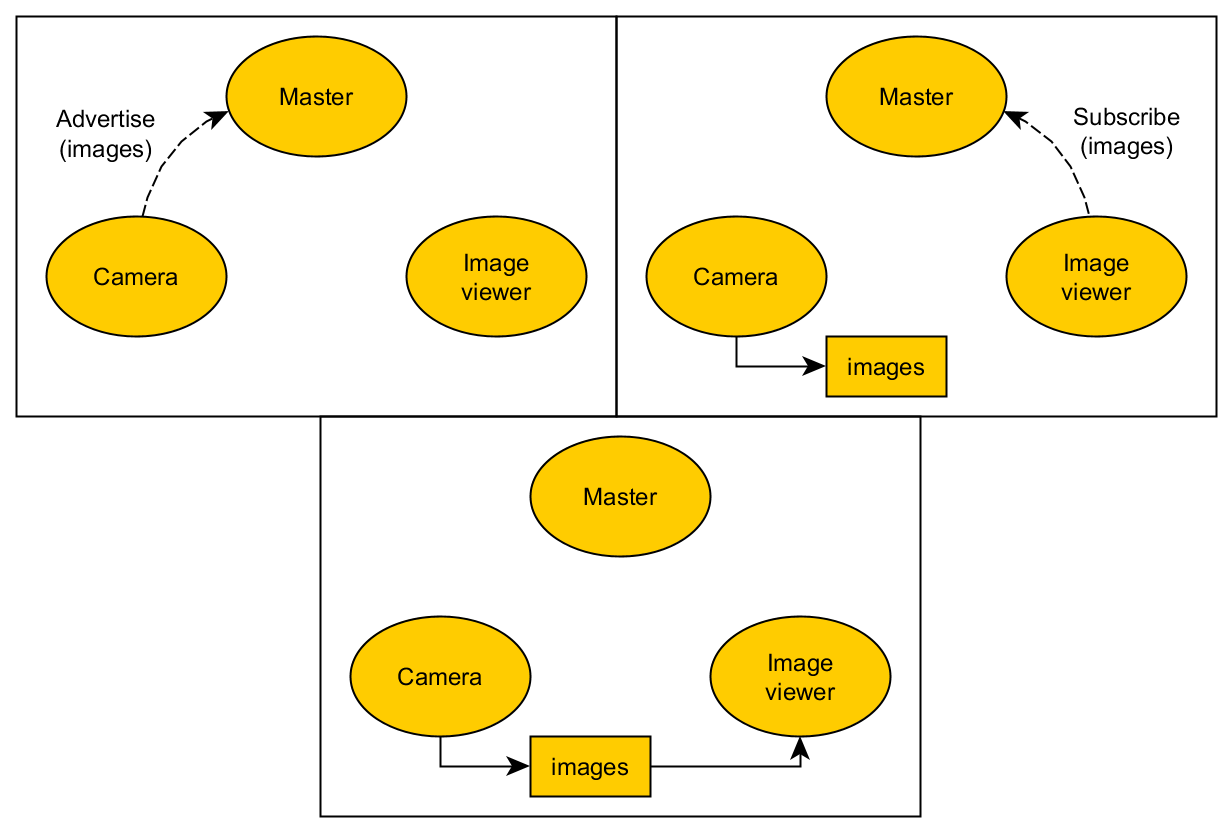
\includegraphics[width=\pictureWidthSmall,keepaspectratio]{graphics/MasterNameserver.png}
	\caption{Der ROS-Master als Nameserver}
	\label{pic:MasterNameserver}
\end{wrapfigure}

Damit die einzelnen Nodes wissen, wo sie ihre Nachrichten hinschicken müssen, gibt es den ROS-Master\footnote{\url{http://wiki.ros.org/Master}}. Diese spezielle Node muss in jedem ROS-System einmal gestartet werden. Sie dient sozusagen als DNS-Server in der Programmumgebung von ROS. Möchte eine Node eine Nachricht an eine andere senden, hat sie nur den Namen der Node. Sie fragt dann den ROS-Master, der ihr die entsprechende Adresse zurück gibt. Aber nicht nur Namen werden vermittelt, sondern auch Topics, wodurch diese dezentral laufen. \autoref{pic:MasterNameserver} zeigt den ROS-Master bei seiner Tätigkeit.

\subsubsection*{Parameter-Server}
Als letztes Modul wird der Parameter-Server vorgestellt\footnote{\url{http://wiki.ros.org/Parameter\%20Server}}. Dieser dient sozusagen als Repository in dem Konfigurationen abgespeichert werden können. Möchte man bestimmte Werte, wie zum Beispiel Preise bei einer Ware, nicht in seinen Programmen hartkodieren um sie flexibel zu halten, kann man sich dem Parameter-Server bedienen. Die Struktur der Parameter ist wie die der Topics \highlight{/camera/left/lens}. Es lassen sich aber ganze Level abfragen, die dann als JSON-ähnliches Format versendet werden.

Der Parameter-Server ist ein Bestandteil des ROS-Masters. Das Abfragen der Parameter setzt also voraus, dass eine Verbindung zu diesem besteht. Entschließt man sich also dazu den Parameter-Server zu nutzen, rückt der ROS-Master wieder ein Stück weiter in den Vordergrund und seine Rolle als kritisches System wird umso stärker. Außerdem erfordert das Abfragen eines Parameters, dass man die TCP/UDP-Verbindung nutzt. Einen Parameter abzufragen ist somit vergleichsweise sehr langsam. Sinnvoller wäre es einen Cache in die eigenen Nodes einzubauen und diesen, entweder über Timer oder Broadcasts über einen Topic manuell, aktualisieren zu lassen.

\subsubsection*{Roslaunch}
Roslaunch ist ein Programm dass es erlaubt mehrere Nodes miteinander zu verketten und als ein Gesamtpaket zu starten\footnote{\url{http://wiki.ros.org/roslaunch}}. Die Pakete werden in einem XML-Format erstellt und bieten besondere Funktionen um die Nodes miteinander zu bündeln und interagieren zu lassen.

Es ist so möglich Nodes mit Parametern\footnote{\url{http://wiki.ros.org/roslaunch/XML/}} zu starten und sie zum Beispiel als \highlight{required} zu kennzeichen. Dies bedeutet, dass alle anderen Nodes die mit dieser im Paket gestartet wurden, sich automatisch abschalten, wenn die betreffende Node sich (freiwillig oder durch Fehler) beendet.
Auch ein umleiten von In- und Output eines Services ist möglich. So lässt sich zum Beispiel ein Logger recht simpel in einer eigenen Node erstellen, der eine Kopie der privaten Inputs und Outputs eines Services kommt um sie zu Loggen. Auch für die Fehlerprüfung ließe sich diese Technik nutzen. Man könnte eine alte Version einer Node mitlaufen lassen und auf diese Weise prüfen, dass die neue Version sich genau so verhält wie die alte (aber performanter ist).